
\begin{center}
{\Large\bfseries Supplementary Information\par}
\vspace{10pt}
{\large\bfseries \PaperTitle\par}
\vspace{12pt}
\AuthorNames\par
\AuthorAffiliations\par
\Correspondence\par
\end{center}
\section*{Contents and source-data guide}
This document contains interpretive notes, twelve supplementary figures and nine supplementary tables. The full architecture and training Methods are now provided in the main article. Supporting source-data exports, including unrounded per-gene observations, accompany the publication package. Independent biological replicates are patients rather than masks or training seeds.
\clearpage
\section{Supplementary notes}
\subsection{Affine interpolation identity}
For a gene with transform $T(y)=(y-\mu)/\sigma$, $\sigma>0$, and interpolation weights satisfying $\sum_j w_{ij}=1$, we have
\begin{align*}
T^{-1}\!\left(\sum_j w_{ij}T(y_j)\right)
&=\sigma\sum_jw_{ij}\frac{y_j-\mu}{\sigma}+\mu\\
&=\sum_j w_{ij}y_j.
\end{align*}
Consequently, applying and inverting a fixed per-gene affine transform does not create a distinct molecular interpolation method when weights are unchanged. In the Wu evaluation, the raw and transformed predictions differed by at most $2.66\times10^{-15}$, consistent with roundoff. Tiny numerical changes can break tied ranks and alter raw Spearman calculations; such changes were logged as numerical rank sensitivity, not counted as harmonization benefits. Calibration can still alter an image branch or a learned fusion model; that is a different comparison. The manuscript therefore omits duplicate molecular interpolation curves and makes no claim of an affine-harmonization advantage for molecular interpolation itself.

\subsection{Dataset roles, masking and interpretation}
The four-patient HEST cohort was used for development. HER2ST was first evaluated under a frozen protocol and subsequently used for calibration development; those two views reuse the same eight patients. The Wu cohort supplied three calibration and three evaluation patients. The 22 Bassiouni patients were evaluated without new cohort-specific fitting. Counts of independent evaluation patients must not add repeated HER2ST analyses or mask replicates as new patients.

Distributed evaluation reveals molecular vectors at sampled anchors and scores all remaining locations. The external regional-completion protocol instead withholds a contiguous 40\% region, samples anchors outside it, and scores that region only. V1 uses inverse-distance-squared interpolation and V2 uses an equal-weight nearest-anchor mean. Their contrast is therefore a protocol-level difference, not an isolated geometry intervention. The earlier development block/capture masks are also not identical to the external forbidden-region design.

Public external H\&E images are downsampled, and sparse molecular interpolation receives same-section expression unavailable to the image-only baseline. Image-resolution limitations and unequal available information must accompany comparisons with histology. An H\&E-fusion failure under these frozen inputs does not establish that native-resolution histology is generally uninformative.

\subsection{Aggregation and metric interpretation}
The primary external summaries compute gene-level metrics on hidden locations, summarize genes within each run, average random seeds within geometry, average geometries within patient, and finally summarize patients. Unless a figure legend states otherwise, external cohort markers are medians across patients. Several development and transportability plots instead show arithmetic means; their legends state this explicitly. A difference between two cohort medians is not a median paired patient effect.

Mean squared error and mean absolute error use the unchanged development-standardized log1p-count target. Shared numerical units do not remove capture-depth or assay differences. Correlations are undefined when the target or prediction range is at most $10^{-12}$; they are excluded from correlation averages but not counted as successes in threshold fractions. Spearman correlations use average ranks for ties. Mask and model seeds describe computational variation, not independent biological replication. No confidence intervals or significance tests have been added.
\clearpage
\section{Supplementary figures}
\begin{figure}[p]
\centering
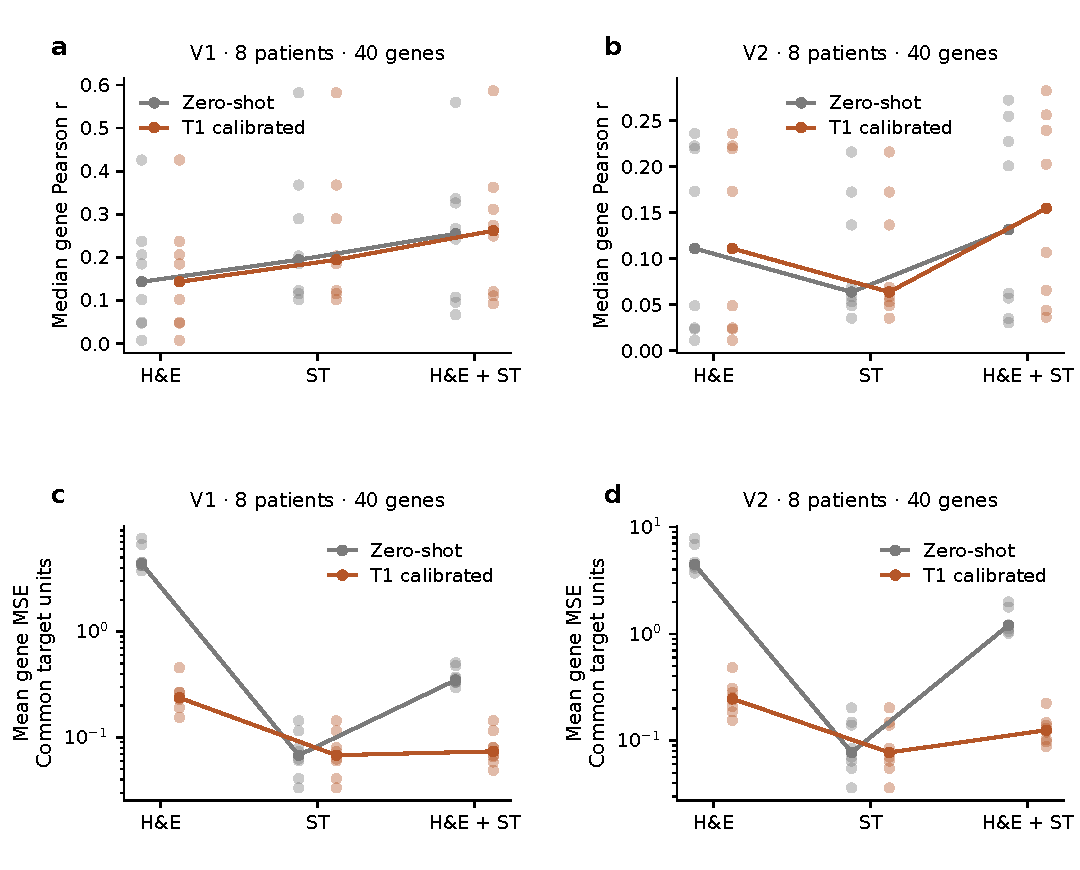
\includegraphics[width=\textwidth,height=0.65\textheight,keepaspectratio]{supplementary_figures/FigureS1.pdf}
\caption{\textbf{HER2ST transportability and target calibration.} Eight HER2ST patients and the frozen 40-gene intersection are shown at 20\% random measured-location coverage. \textbf{a,c,} Distributed interpolation (V1). \textbf{b,d,} Contiguous regional completion (V2). Panels a/b show median gene Pearson correlation and c/d show mean gene MSE in common target units on a logarithmic axis. Dots are patient summaries after averaging seeds and geometries; connected markers are medians across patients. T0 denotes the uncalibrated zero-shot analysis, whereas T1 denotes the calibrated target mapping with fixed fusion. Image weights were 0.25 for V1 and 0.5 for V2; these development weights differ from the final external weight of 0.2. These are the same patients, not independent replication groups. The T1 fixed-fusion analysis differs from the later fold-selected fusion results in Supplementary Fig.~S10. Affine transformation and inverse transformation leave molecular interpolation unchanged; apparent image/fusion calibration effects are not a new interpolation advantage.}
\label{fig:s1}
\end{figure}\clearpage
\begin{figure}[p]
\centering
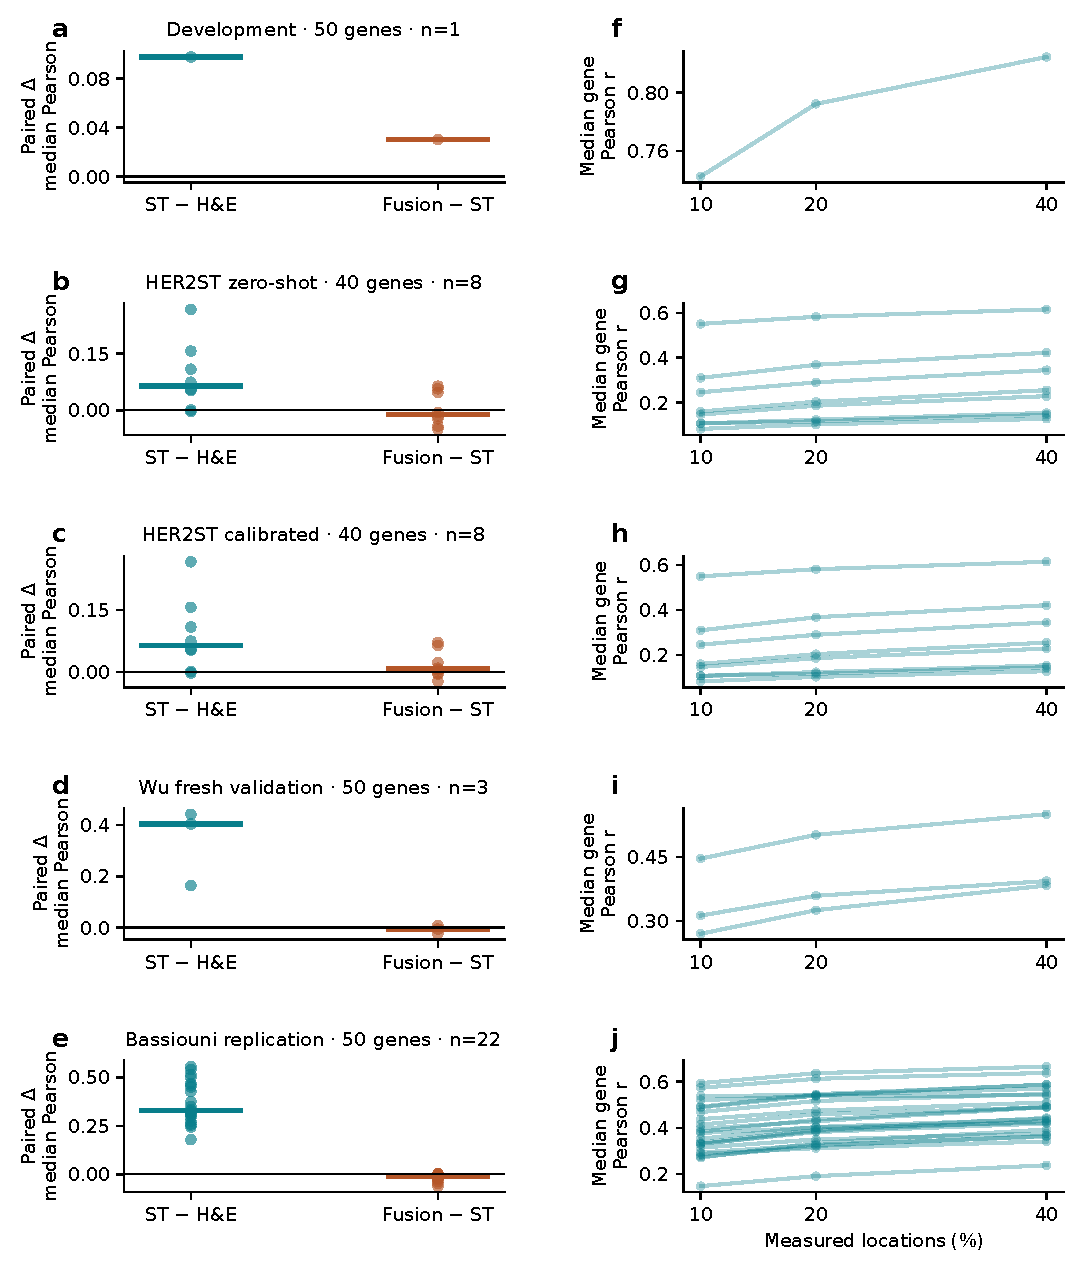
\includegraphics[width=\textwidth,height=0.80\textheight,keepaspectratio]{supplementary_figures/FigureS2.pdf}
\caption{\textbf{Cross-cohort synthesis without pooling different panels.} Rows correspond to the development primary patient ($n=1$), HER2ST zero-shot ($n=8$), HER2ST calibrated ($n=8$, the same patients), fresh Wu evaluation ($n=3$) and fresh Bassiouni replication ($n=22$). The development and fresh cohorts use 50 genes; HER2ST uses 40. \textbf{a--e,} Left-column paired patient correlation effects at 20\% distributed coverage for molecular interpolation minus image-only prediction and fusion minus molecular interpolation; bars are median paired effects. \textbf{f--j,} Right-column individual patient molecular correlation curves at 10\%, 20\% and 40\% distributed coverage. The panels preserve differences in analytical role and gene panel and do not define a pooled cross-cohort score. HER2ST calibration is development, not an additional fresh validation cohort.}
\label{fig:s2}
\end{figure}\clearpage
\begin{figure}[p]
\centering
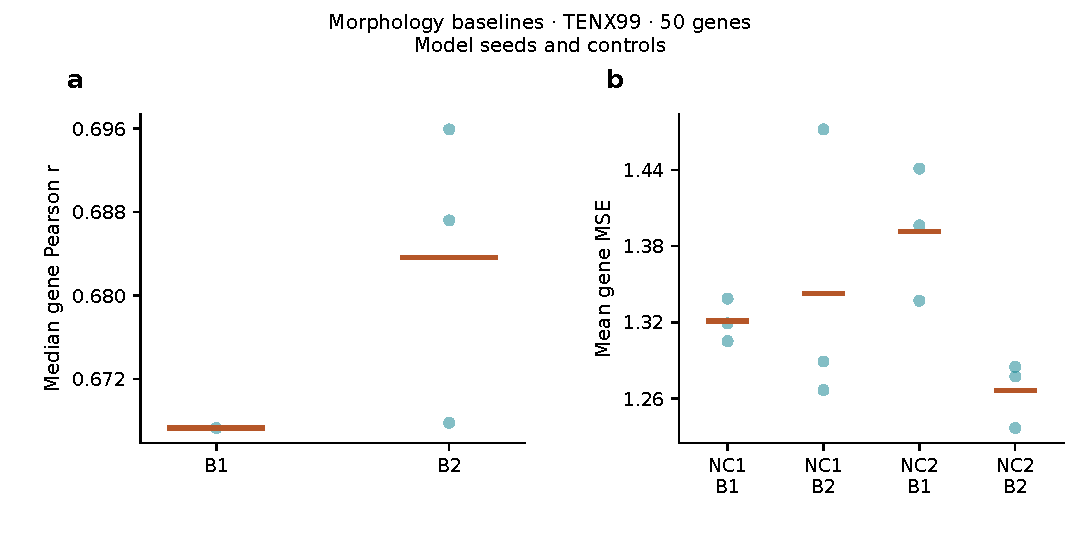
\includegraphics[width=\textwidth,height=0.65\textheight,keepaspectratio]{supplementary_figures/FigureS3.pdf}
\caption{\textbf{Morphology-only development baselines and controls.} The morphology-only development analyses use the single primary development patient TENX99 and 50 genes. \textbf{a,} Median gene Pearson correlation for ridge regression (B1) and the small multilayer perceptron (B2). The training-mean baseline has constant predictions and undefined correlations and is not drawn as zero. \textbf{b,} MSE under training-target-row permutation (NC1) and training-embedding-row permutation (NC2). Dots represent saved model-seed runs and bars are arithmetic means of displayed runs, not independent patient estimates. The controls disrupt image--expression pairing while preserving validation and evaluation data. This initial image-only head differs from the frozen local MLP selected in the representation comparison and used for external replication.}
\label{fig:s3}
\end{figure}\clearpage
\begin{figure}[p]
\centering
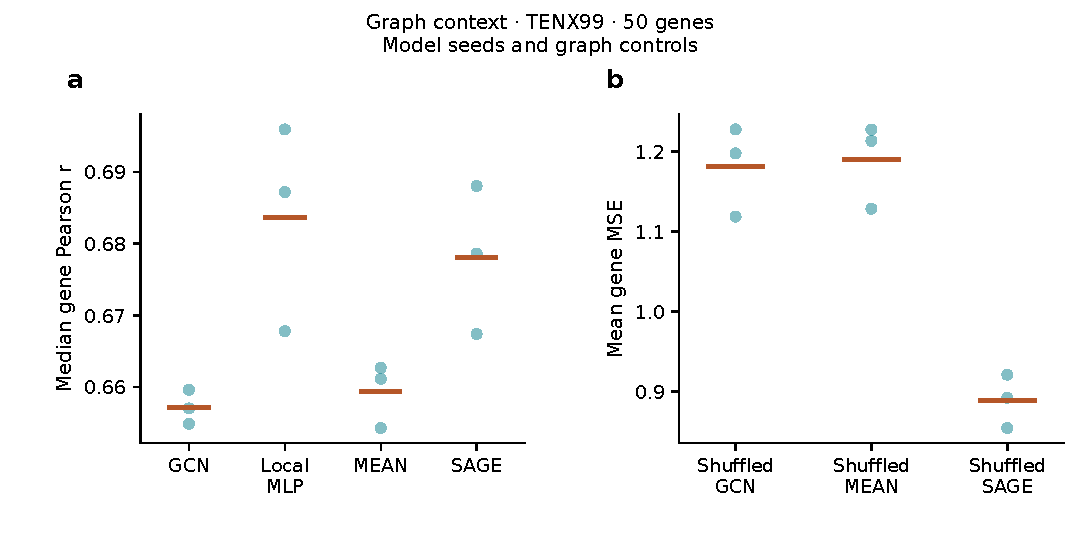
\includegraphics[width=\textwidth,height=0.65\textheight,keepaspectratio]{supplementary_figures/FigureS4.pdf}
\caption{\textbf{Single-scale graph context did not by itself establish spatial specificity.} The single-scale graph comparison uses TENX99 and the 50-gene panel. \textbf{a,} Median gene correlation for the frozen local MLP, neighborhood mean pooling plus MLP, GCN and GraphSAGE. \textbf{b,} Mean gene MSE for the archived shuffled-neighborhood runs. Dots are training-seed runs and bars are their arithmetic means. A graph model outperforming a local predictor does not establish that the correct spatial adjacency caused the gain; generic aggregation or model parameterization can also contribute. The results use the original fitted models without additional graph selection or local-predictor refitting.}
\label{fig:s4}
\end{figure}\clearpage
\begin{figure}[p]
\centering
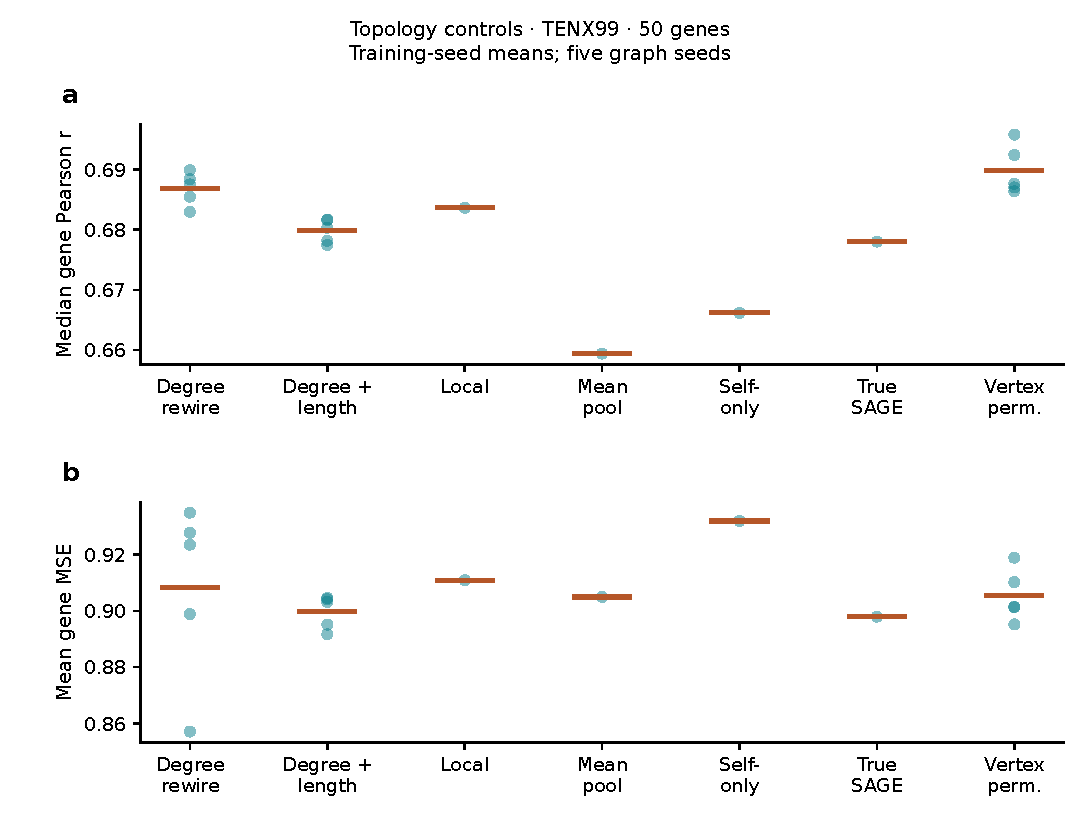
\includegraphics[width=\textwidth,height=0.65\textheight,keepaspectratio]{supplementary_figures/FigureS5.pdf}
\caption{\textbf{Matched graph controls limited claims about exact topology.} The matched graph controls use one development patient, TENX99, and 50 genes. \textbf{a,} Median gene Pearson correlation. \textbf{b,} Mean gene MSE. Local, self-only, mean-pooling and true-spatial GraphSAGE results accompany vertex-permuted, degree-rewired and degree-plus-edge-length-rewired controls. Training seeds are averaged within each graph randomization seed; the randomized controls have five graph seeds. Dots are these averages and bars are arithmetic means. Random graph seeds are not biological replicates. The experiment did not establish a reproducible advantage of the true spatial topology. This figure records a negative/mixed development result, not evidence that topology is irrelevant in every representation or tissue.}
\label{fig:s5}
\end{figure}\clearpage
\begin{figure}[p]
\centering
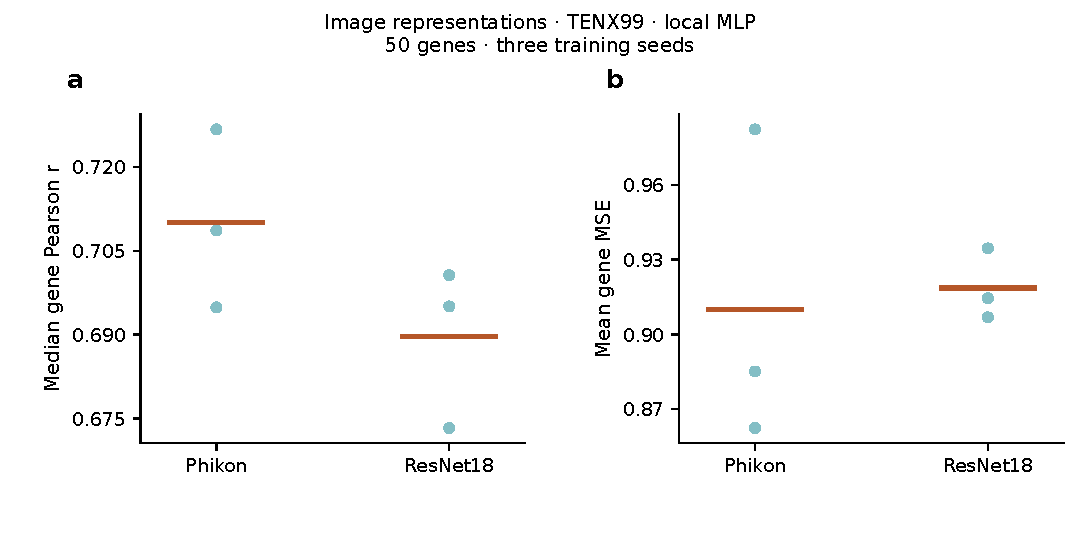
\includegraphics[width=\textwidth,height=0.65\textheight,keepaspectratio]{supplementary_figures/FigureS6.pdf}
\caption{\textbf{Pathology representation effects in the development patient.} The local MLP representation comparison evaluates frozen ImageNet ResNet18 and Phikon representations in TENX99 for 50 genes. \textbf{a,} Median gene Pearson correlation. \textbf{b,} Mean gene MSE. Each dot is one of three training seeds; bars are arithmetic means. The panel-specific improvement did not establish general superiority on larger target panels or reproducible topology-specific gains. Phikon is not introduced into the final Bassiouni replication; that analysis retains the frozen ResNet18 image branch. These are development comparisons, not external encoder validation.}
\label{fig:s6}
\end{figure}\clearpage
\begin{figure}[p]
\centering
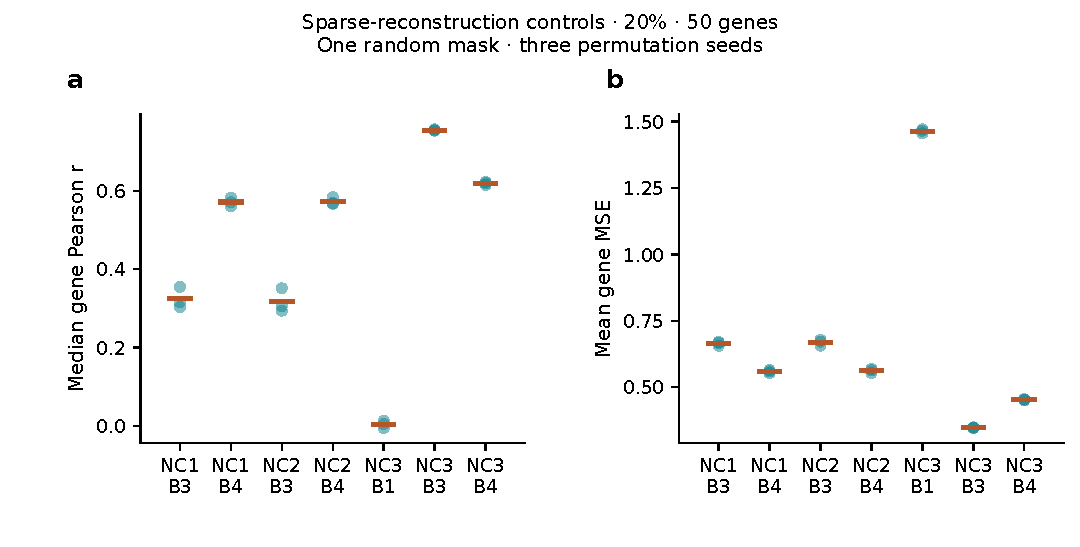
\includegraphics[width=\textwidth,height=0.65\textheight,keepaspectratio]{supplementary_figures/FigureS7.pdf}
\caption{\textbf{Sparse-reconstruction development controls.} The sparse-reconstruction controls use the ResNet18 branch, TENX99, 50 genes and 20\% measured-location coverage. In this figure, B1 denotes image-only prediction, B3 image--molecular fusion and B4 learned propagation. Controls include anchor-expression permutation (NC1), anchor-position permutation (NC2) and image-location permutation (NC3). Model labels are specific to this experiment. \textbf{a,} Median gene Pearson correlation. \textbf{b,} Mean gene MSE. All controls use the same random observation mask (replicate 0); dots represent three permutation seeds and bars are arithmetic means. These distributions are control diagnostics rather than estimates of a geometry effect. Separate integrity checks establish invariance to corruption of hidden labels. Related anchor-assignment disruptions must not be counted as independent biological mechanisms.}
\label{fig:s7}
\end{figure}\clearpage
\begin{figure}[p]
\centering
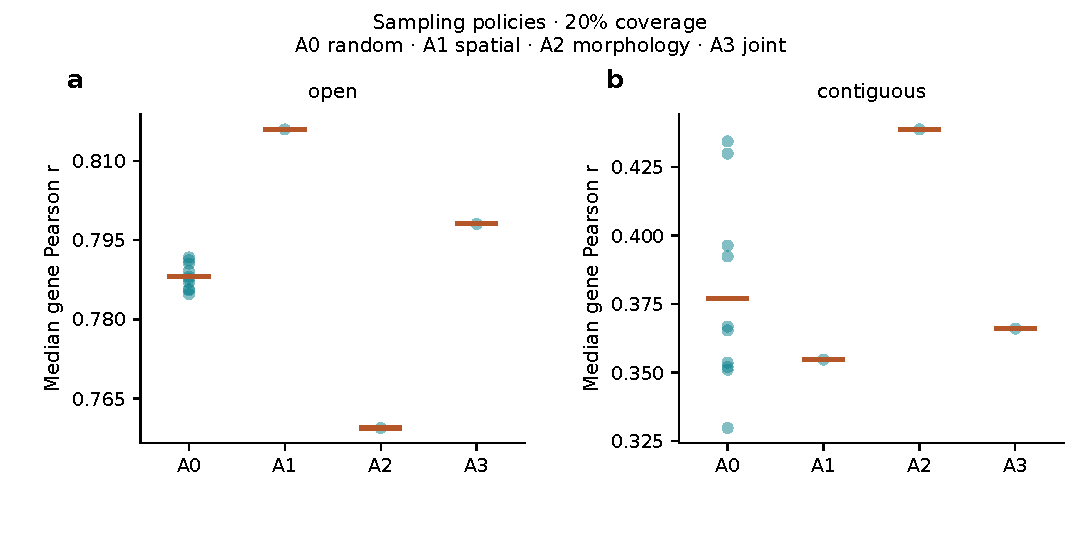
\includegraphics[width=\textwidth,height=0.65\textheight,keepaspectratio]{supplementary_figures/FigureS8.pdf}
\caption{\textbf{Sampling effects depended on the reconstruction regime.} The sampling comparison uses interpolation-only results for TENX99, the ResNet18 reference branch, 50 genes and 20\% coverage. \textbf{a,} Open-tissue interpolation. \textbf{b,} Contiguous missing-region evaluation. A0 is random sampling with ten seeds; A1 is spatial farthest-point sampling, A2 morphology-space farthest-point sampling, and A3 a locked joint policy. A1--A3 are deterministic given their stored initialization. Dots are policy runs and bars are arithmetic means. This limited baseline diagnostic is not a complete summary of all learned/fusion families and does not demonstrate universally optimal sampling.}
\label{fig:s8}
\end{figure}\clearpage
\begin{figure}[p]
\centering
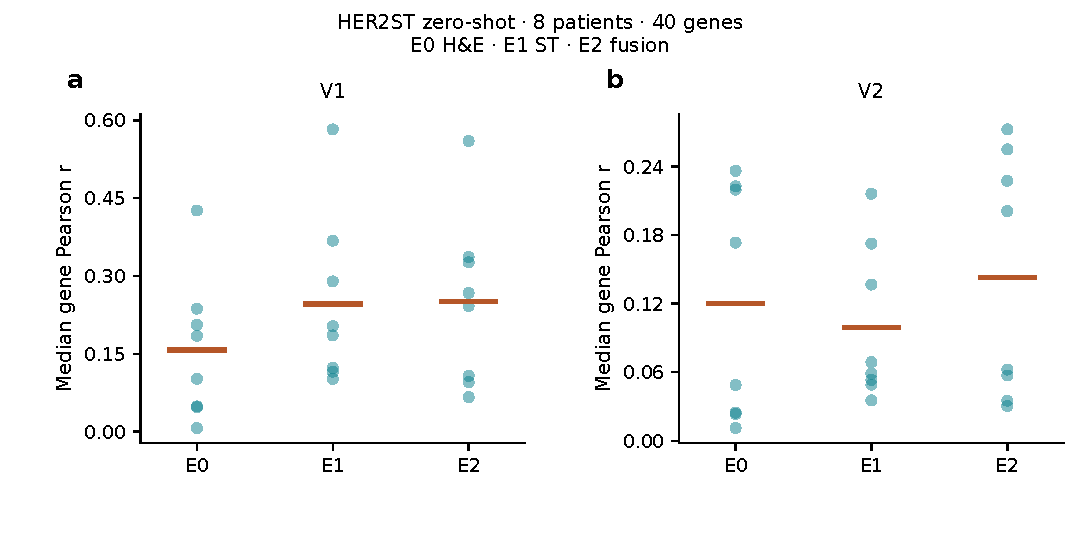
\includegraphics[width=\textwidth,height=0.65\textheight,keepaspectratio]{supplementary_figures/FigureS9.pdf}
\caption{\textbf{HER2ST patient distributions under the frozen zero-shot protocol.} The eight HER2ST patients, 40 shared primary genes and 20\% random-anchor coverage are summarized separately for \textbf{a,} distributed interpolation and \textbf{b,} contiguous regional completion. E0 denotes H\&E-only prediction, E1 molecular interpolation and E2 frozen fusion, with image weights 0.25 for V1 and 0.5 for V2. Dots are patient means across seeds/geometries. Bars are arithmetic patient means, unlike the median summaries in Supplementary Fig.~S1 and the primary tables. These zero-shot results and the subsequent calibration analyses use the same patients; HER2ST therefore does not supply an untouched final validation cohort.}
\label{fig:s9}
\end{figure}\clearpage
\begin{figure}[p]
\centering
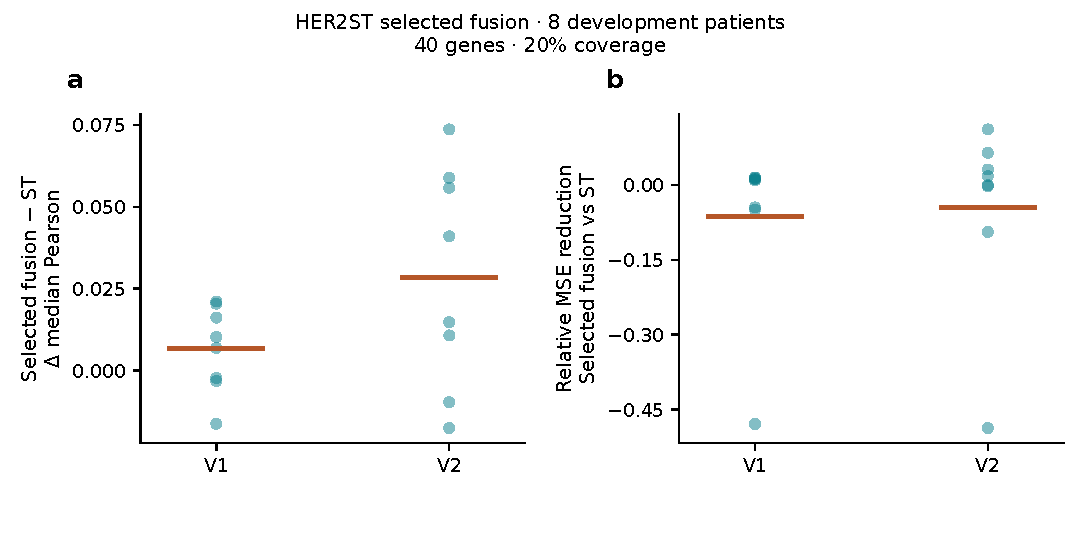
\includegraphics[width=\textwidth,height=0.65\textheight,keepaspectratio]{supplementary_figures/FigureS10.pdf}
\caption{\textbf{Patient-disjoint calibration did not establish robust fusion superiority.} The calibration-development analysis includes eight HER2ST patients, the frozen 40-gene intersection and 20\% coverage. \textbf{a,} Selected calibrated fusion minus molecular interpolation in Pearson correlation. \textbf{b,} Relative MSE reduction compared with molecular interpolation; positive values indicate lower fusion error. Dots are patient/fold results grouped by V1/V2 and bars are arithmetic means. The selected fusion rule was determined within patient-disjoint training/calibration folds, not from the displayed outer-patient outcomes. Joint correlation and error improvements were not consistent across patients. These selected-fusion results should not be interchanged with the T1 fixed-fusion target study shown in Supplementary Fig.~S1.}
\label{fig:s10}
\end{figure}\clearpage
\begin{figure}[p]
\centering
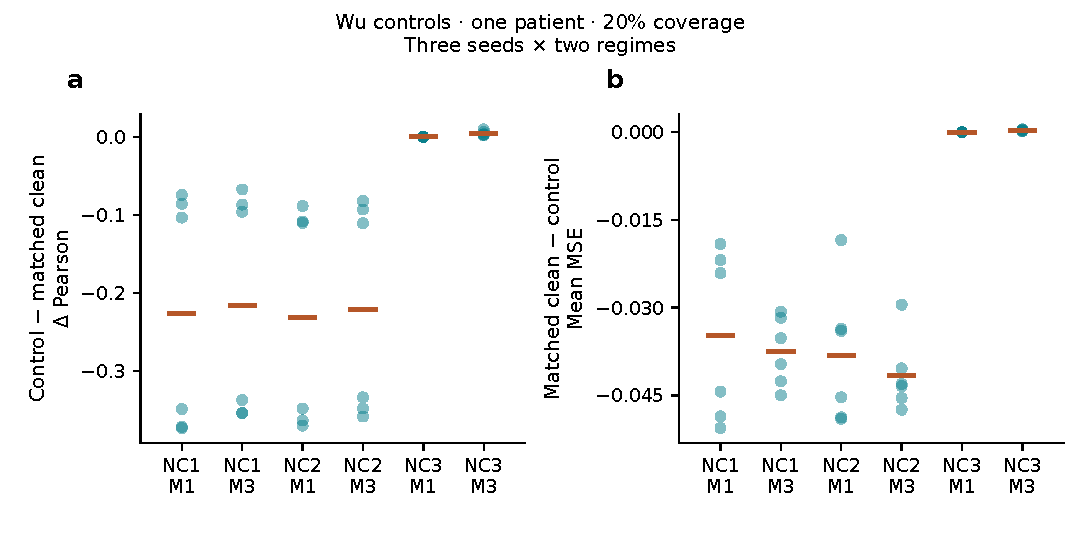
\includegraphics[width=\textwidth,height=0.65\textheight,keepaspectratio]{supplementary_figures/FigureS11.pdf}
\caption{\textbf{Matched negative controls in fresh Wu evaluation.} The predeclared held-out patient 1160920F, 50 genes, 20\% coverage and random mask seed 0 were used, with V1 geometry 0 and V2 geometry 1. Three permutation seeds were evaluated for NC1 anchor-vector reassignment, NC2 anchor-position reassignment and NC3 image-prediction permutation. \textbf{a,} Control minus matched-clean median gene Pearson correlation. \textbf{b,} Matched-clean minus control MSE, so negative values indicate increased control error. Molecular interpolation (M1) and fixed image fusion (M3) are shown. Dots are matched control settings and bars are means; they are not independent patients. Molecular controls disrupt the correct spatial anchor assignments, whereas image permutation provides no robust supporting evidence for the frozen image contribution.}
\label{fig:s11}
\end{figure}\clearpage
\begin{figure}[p]
\centering
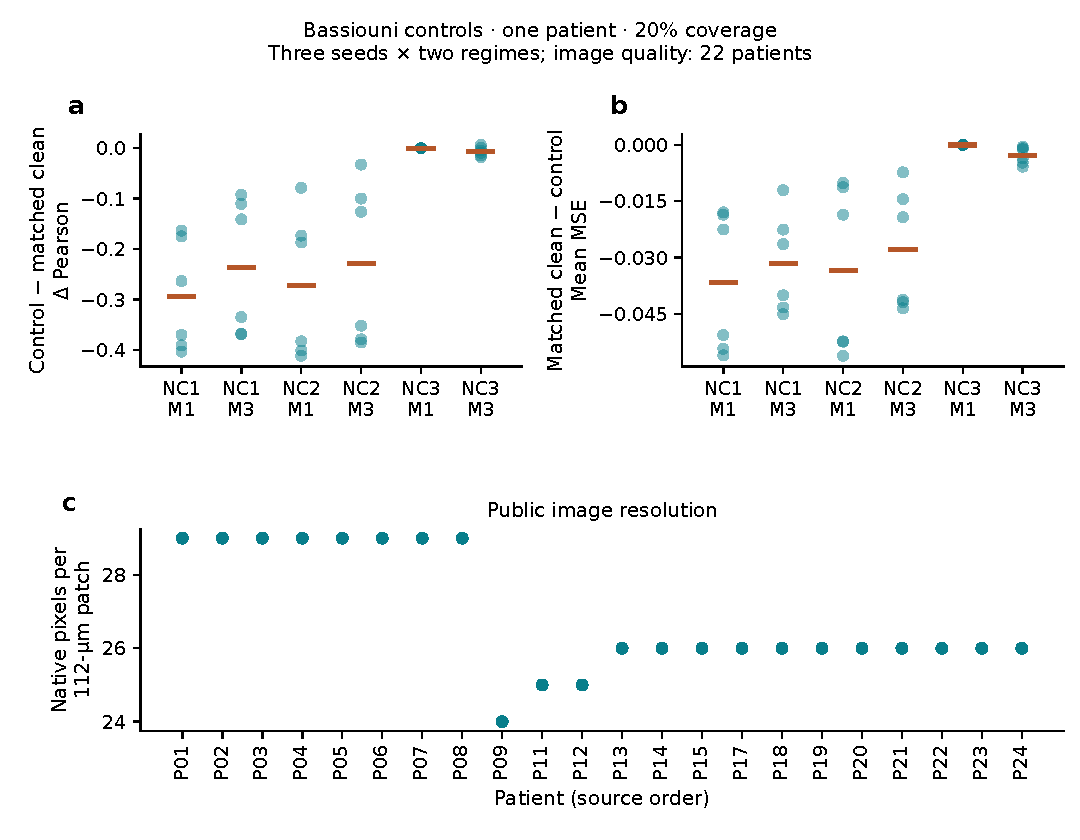
\includegraphics[width=\textwidth,height=0.65\textheight,keepaspectratio]{supplementary_figures/FigureS12.pdf}
\caption{\textbf{Replication controls and native image resolution.} The independent-replication controls use the predeclared Bassiouni patient BASS\_P01, 50 genes, 20\% coverage, random mask seed 0, V1 geometry 0 and V2 geometry 1. \textbf{a,b,} Matched Pearson and MSE effects for M1/M3 under three control seeds, with definitions and signs as in Supplementary Fig.~S11. Dots are matched control settings and bars are arithmetic means. \textbf{c,} Native pixels per nominal 112-\um{} patch for all 22 patients in source order. The supplied images provide only 24--29 native pixels before resizing for the encoder. This is image-input quality control, not expression-prediction performance. It explains why the image comparisons cannot establish the limits of native-resolution histopathology. Coordinate overlays for all patients are recorded in the archived qualification audit.}
\label{fig:s12}
\end{figure}\clearpage
\section{Supplementary tables}
The tables below provide compact views of the accompanying machine-readable data and definitions needed to interpret the supplementary figures. Table~S2 is rounded for presentation; the digital files retain unrounded exported values. Large gene-level and distance-resolved tables are supplied as separate files rather than reproduced in full in this PDF. Mask, model and permutation seeds are computational replicates and do not increase the number of independent patients.
\begin{table}[htbp]
\caption{\textbf{Primary gene panel.} The 50 genes are listed in the order fixed by variance ranking in the development-training patients. The fresh Wu and Bassiouni analyses retain all 50 genes. HER2ST analyses use the 40-gene intersection with this panel; unavailable genes are not replaced. The full data file also includes the larger development panels and cohort-specific availability records: \protect\path{source_data/SuppTable1_gene_panels.csv}.}
\centering\small
\begin{tabular}{rlrl}\toprule
Order & Gene & Order & Gene\\\midrule
1 & FOXA1 & 26 & LUM \\
2 & SCD & 27 & MYO5B \\
3 & KRT7 & 28 & SFRP4 \\
4 & ERBB2 & 29 & KRT14 \\
5 & POSTN & 30 & TOP2A \\
6 & CEACAM6 & 31 & IL7R \\
7 & SERHL2 & 32 & AR \\
8 & ANKRD30A & 33 & KRT5 \\
9 & EPCAM & 34 & PCLAF \\
10 & ABCC11 & 35 & KLF5 \\
11 & TACSTD2 & 36 & SFRP1 \\
12 & GATA3 & 37 & TRAF4 \\
13 & FASN & 38 & CXCR4 \\
14 & MLPH & 39 & MYH11 \\
15 & S100A14 & 40 & TENT5C \\
16 & CDH1 & 41 & TCIM \\
17 & CD9 & 42 & NARS \\
18 & KRT8 & 43 & ACTG2 \\
19 & CCND1 & 44 & PDK4 \\
20 & DSP & 45 & CD3E \\
21 & SERPINA3 & 46 & TRAC \\
22 & LYPD3 & 47 & JUP \\
23 & TFAP2A & 48 & LYZ \\
24 & TPD52 & 49 & CENPF \\
25 & PTGDS & 50 & CCDC80 \\
\bottomrule\end{tabular}\end{table}\clearpage
\begin{table}[p]
\caption{\textbf{Patient-resolved reconstruction metrics.} Compact view of the 25 fresh evaluation patients at 20\% distributed coverage, using 50 genes. Values average mask seeds within patient. $r$ is the median gene Pearson correlation; MSE is mean gene squared error in the common target units. I denotes image-only, ST molecular interpolation, and F fixed image fusion. Complete exported patient summaries for the available cohorts, regimes, budgets and methods are supplied in \protect\path{source_data/SuppTable2_per_patient.csv}.}
\centering\small
\begin{tabular}{lrrrrrr}\toprule
Patient & $r_{\mathrm I}$ & $r_{\mathrm{ST}}$ & $r_{\mathrm F}$ & MSE$_{\mathrm I}$ & MSE$_{\mathrm{ST}}$ & MSE$_{\mathrm F}$\\\midrule
\multicolumn{7}{l}{\textit{Wu}}\\
1160920F & -0.045 & 0.359 & 0.335 & 0.846 & 0.082 & 0.095\\
CID4290 & 0.161 & 0.325 & 0.333 & 2.915 & 0.099 & 0.100\\
CID44971 & 0.059 & 0.502 & 0.496 & 2.949 & 0.115 & 0.118\\
\multicolumn{7}{l}{\textit{Bassiouni}}\\
BASS\_P01 & 0.077 & 0.382 & 0.370 & 1.304 & 0.087 & 0.106\\
BASS\_P02 & 0.009 & 0.459 & 0.431 & 1.067 & 0.093 & 0.127\\
BASS\_P03 & 0.030 & 0.545 & 0.537 & 2.585 & 0.081 & 0.089\\
BASS\_P04 & -0.039 & 0.334 & 0.312 & 1.882 & 0.113 & 0.125\\
BASS\_P05 & 0.096 & 0.636 & 0.628 & 1.581 & 0.133 & 0.155\\
BASS\_P06 & -0.005 & 0.312 & 0.297 & 1.567 & 0.069 & 0.072\\
BASS\_P07 & 0.013 & 0.191 & 0.180 & 2.684 & 0.092 & 0.097\\
BASS\_P08 & 0.095 & 0.403 & 0.393 & 2.120 & 0.088 & 0.095\\
BASS\_P09 & 0.075 & 0.391 & 0.380 & 1.763 & 0.120 & 0.139\\
BASS\_P11 & -0.081 & 0.474 & 0.464 & 2.052 & 0.104 & 0.109\\
BASS\_P12 & 0.182 & 0.435 & 0.436 & 1.748 & 0.113 & 0.120\\
BASS\_P13 & 0.151 & 0.612 & 0.615 & 2.228 & 0.104 & 0.119\\
BASS\_P14 & 0.041 & 0.540 & 0.536 & 1.458 & 0.126 & 0.154\\
BASS\_P15 & 0.093 & 0.386 & 0.389 & 1.777 & 0.101 & 0.115\\
BASS\_P17 & 0.095 & 0.428 & 0.421 & 1.773 & 0.088 & 0.096\\
BASS\_P18 & 0.090 & 0.516 & 0.496 & 2.391 & 0.083 & 0.086\\
BASS\_P19 & 0.068 & 0.537 & 0.501 & 2.431 & 0.068 & 0.078\\
BASS\_P20 & 0.067 & 0.326 & 0.319 & 2.407 & 0.096 & 0.098\\
BASS\_P21 & 0.075 & 0.401 & 0.340 & 2.607 & 0.092 & 0.108\\
BASS\_P22 & -0.029 & 0.322 & 0.300 & 2.149 & 0.087 & 0.090\\
BASS\_P23 & 0.267 & 0.541 & 0.525 & 2.166 & 0.054 & 0.061\\
BASS\_P24 & 0.106 & 0.350 & 0.302 & 1.626 & 0.048 & 0.052\\
\bottomrule\end{tabular}
\end{table}\clearpage
\begin{table}[htbp]
\caption{\textbf{Per-gene results and metric definitions.} The accompanying digital table, \protect\path{source_data/SuppTable3_per_gene.csv.gz}, contains the exported Wu and Bassiouni gene-level results, with run, patient, panel, mask and method identifiers. Compression changes storage only. Every metric is calculated using the hidden locations scored by the corresponding protocol. The definitions below explain the gene-level statistics and their summaries; genes and repeated runs are not independent patient observations.}
\label{tab:s3}
\centering\small
\begin{tabularx}{\textwidth}{>{\RaggedRight\arraybackslash}p{0.23\textwidth}Y}\toprule
Quantity & Definition and interpretation\\\midrule
Pearson correlation & Correlation between predicted and measured values across scored locations, calculated separately for each gene. Constant targets or predictions yield undefined correlations.\\
Spearman correlation & Correlation between the ranks of predicted and measured values across scored locations, calculated separately for each gene. Numerical changes in tied ranks do not establish a biological improvement.\\
Mean squared error (MSE) & Mean squared prediction error across scored locations for each gene, evaluated in the common development-standardized log1p-count units.\\
Mean absolute error (MAE) & Mean absolute prediction error across scored locations for each gene, evaluated in the same target units.\\
Panel correlation & Median of defined gene correlations. Undefined correlations are excluded from this median and do not count as positive-correlation successes.\\
Panel error & Arithmetic mean of the gene-level MSEs or MAEs. All genes are retained in error summaries.\\
Patient and cohort summaries & Mask seeds are averaged within geometry and geometries within patient. Headline cohort values are medians of patient summaries; paired effects are calculated within patients before summarizing them.\\
\bottomrule\end{tabularx}
\end{table}
\begin{table}[htbp]
\caption{\textbf{Negative-control families.} Control definitions are experiment-specific and are given in the corresponding figure legends. Training-row controls differ from inference-time controls that permute permitted sparse inputs. Permuting anchor-expression assignments and anchor-position assignments disrupts related associations and does not constitute independent biological evidence. Exported control results are supplied in \protect\path{source_data/SuppTable4_negative_controls.csv}.}
\label{tab:s4}
\centering\small
\begin{tabularx}{\textwidth}{>{\RaggedRight\arraybackslash}p{0.28\textwidth}Y}\toprule
Control family & Interpretation\\\midrule
Training-target or training-embedding row permutation & Disrupts local morphology--target pairing during development while preserving the validation and evaluation data.\\
Anchor-expression assignment permutation & Reassigns observed expression vectors among anchors, disrupting their correspondence with spatial position.\\
Anchor-position assignment permutation & Disrupts the spatial assignment of observed anchors while retaining the permitted molecular information.\\
Image-location or image-prediction permutation & Tests dependence on the image input while retaining the allowed molecular measurements.\\
\bottomrule\end{tabularx}
\end{table}\clearpage
\begin{table}[htbp]
\caption{\textbf{Recorded integrity and replay checks.} Counts are taken from the original Wu and Bassiouni technical audits; these audits were not rerun during manuscript preparation. Method predictions and metric arrays are distinct audit units. For each prediction, hidden labels were independently replaced by NaNs and random values to test that unobserved expression could not influence model inputs. Digital records: \protect\path{source_data/SuppTable5_integrity.csv}.}
\label{tab:s5}
\centering\small
\begin{tabular}{lrr}\toprule
Audit quantity & Wu & Bassiouni\\\midrule
Mask trajectories & 132 & 968\\
Clean run bundles & 396 & 2,904\\
Control run bundles & 18 & 18\\
Method prediction replays & 1,656 & 8,766\\
Metric array replays & 6,624 & 35,064\\
Hidden-label corruption checks & 3,312 & 17,532\\
\bottomrule\end{tabular}
\end{table}
\begin{table}[htbp]
\caption{\textbf{Observation masks and sampling protocols.} Coverage is the proportion of retained locations with observed complete expression vectors, not the proportion of tissue area assayed. All unobserved labels are excluded from model inputs. The three regional geometries and ten random-mask seeds are computational replicates. The accompanying \protect\path{source_data/SuppTable6_masks.csv} records the exported mask identities, patients, regimes, geometries and sampling trajectories.}
\label{tab:s6}
\centering\small
\begin{tabularx}{\textwidth}{>{\RaggedRight\arraybackslash}p{0.28\textwidth}Y}\toprule
Protocol component & Definition\\\midrule
Measurement budgets & For $N$ retained locations and $b\in\{0.10,0.20,0.40\}$, the observed count is $\lfloor bN+0.5\rfloor$. Random anchor sets use nested prefixes of the same trajectory as coverage increases.\\
Distributed interpolation (V1) & Anchors may be sampled throughout the retained tissue; every remaining location is scored. Predictions use up to 16 nearest observed anchors with normalized inverse-distance-squared weights.\\
Contiguous regional completion (V2) & A prespecified contiguous region contains the 40\% of locations nearest to its center. Anchors are sampled outside that region, and only locations within it are scored. Predictions use the mean of up to 16 nearest observed anchors.\\
Regional geometry & Three centers are selected at the 25th, 50th and 75th percentile of first coordinate principal-component rank. The three geometries are averaged equally within patient.\\
Secondary spatial sampling & Label-free farthest-point sampling starts from the eligible location farthest from the eligible-coordinate centroid. It is not optimized using external expression outcomes.\\
Development masks & Earlier block and capture-window masks differ from the external regional-completion protocol and are interpreted separately.\\
\bottomrule\end{tabularx}
\end{table}\clearpage
\begin{table}[htbp]
\caption{\textbf{Distance-resolved evaluation and patient support.} Distance is measured from each scored hidden location to its nearest observed anchor. Empty bins are omitted. Bassiouni binwise Pearson correlations require at least 20 scored locations in the corresponding run; Wu distance bins report MSE and MAE only. Error summaries may include smaller occupied bins. The patient counts below summarize the Bassiouni cohort at 20\% coverage and do not define a universal distance cutoff. Exported bin-level metrics and support counts are supplied in \protect\path{source_data/SuppTable7_distance_bins.csv}.}
\label{tab:s7}
\centering\small
\begin{tabularx}{\textwidth}{>{\RaggedRight\arraybackslash}p{0.34\textwidth}Y}\toprule
Evaluation component & Definition\\\midrule
Distance bins (\um) & $[0,150)$, $[150,300)$, $[300,600)$, $[600,1200)$, $[1200,2400)$ and $[2400,\infty)$.\\
Bin support & Number of scored hidden locations contributing to the patient, method, mask and distance-bin summary; occupied-bin support may differ across patients and protocols.\\
Nearest-to-farthest comparison & Compares MSE in the nearest and farthest occupied bins within each patient.\\
Monotonicity & Assesses whether MSE strictly increases across the occupied distance bins.\\
\bottomrule\end{tabularx}
\vspace{12pt}
\begin{tabularx}{\textwidth}{Yrr}\toprule
Bassiouni patient summary & V1 & V2\\\midrule
Higher MSE in farthest than nearest occupied bin & 15/22 & 20/22\\
Strictly increasing occupied-bin MSE & 6/22 & 13/22\\
\bottomrule\end{tabularx}
\end{table}
\clearpage
\begin{table}[p]
\caption{\textbf{Selected supporting predictor architectures for the 50-gene panel.} Dimensions denote input $\rightarrow$ hidden $\rightarrow$ output, and every listed MLP has GELU, dropout 0.1 and a linear output layer. Encoder parameters remain frozen; counts include trainable head biases. All MLPs use the shared optimizer and stopping rule above. The initial local predictor and the representation-comparison predictor are distinct fitted heads.}
\label{tab:supporting_architectures}
\centering\small
\begin{tabularx}{\textwidth}{@{}>{\RaggedRight\arraybackslash}p{0.25\textwidth}>{\RaggedRight\arraybackslash}p{0.22\textwidth}Y@{}}
\toprule
Predictor & Selected dimensions & Fitting settings or fixed aggregation\\
\midrule
Initial ResNet18 ridge & $512\rightarrow50$ & Ridge penalty 100; intercept; 25,650 coefficients.\\
Initial ResNet18 MLP & $512\rightarrow128\rightarrow50$ & Lowest validation MSE; 72,114 head parameters.\\
ResNet18 mean pooling / GCN & $512\rightarrow128\rightarrow50$ & $PX$ or $QX$ on capped Delaunay adjacency; 72,114 head parameters.\\
ResNet18 mean-GraphSAGE & $1024\rightarrow67\rightarrow50$ & $[X,RX]$ on capped Delaunay adjacency; 72,075 head parameters.\\
ResNet18 representation-comparison MLP & $512\rightarrow256\rightarrow50$ & Highest validation median gene Pearson; 144,178 head parameters.\\
Phikon local MLP & $768\rightarrow256\rightarrow50$ & Same candidate grid and selection criterion; 209,714 head parameters.\\
Phikon spatial MLPs & $768\rightarrow128\rightarrow50$; $1536\rightarrow67\rightarrow50$ & Mean pooling and mean-GraphSAGE, respectively; inherited graph and head widths.\\
Sparse residual correction & 34 covariates plus intercept per gene & Gene-specific ridge correction of fixed fusion; penalty 10,000; 1,750 coefficients for 50 genes.\\
\bottomrule
\end{tabularx}
\end{table}

\clearpage
\begin{table}[!htbp]
\caption{\textbf{Coverage response and contiguous-region completion in the two fresh studies.} All rows use the same frozen 50-gene panel and spatial interpolation. Values are medians of patient summaries, with $n=3$ for Wu and $n=22$ for Bassiouni. V1 is distributed interpolation with inverse-distance-squared weighting; V2 is completion of a predefined contiguous region using the mean of nearby anchors. Both the scoring support and interpolation rule change between V1 and V2. The comparison therefore describes protocol-level deterioration rather than an isolated causal geometry effect. In both studies, every evaluation patient improved in Pearson correlation and MSE from 10\% to 40\% V1 coverage; every patient deteriorated in Pearson, MSE and MAE under V2 relative to V1 at 20\%.}
\label{tab:coverage}
\centering\small
\begin{tabularx}{\textwidth}{@{}Yrrrrr@{}}
\toprule
Cohort & Coverage & V1 Pearson $r$ & V1 MSE & V2 Pearson $r$ & V2 MSE \\
\midrule
Wu, fresh & 10\% & 0.313 & 0.1080 & 0.111 & 0.1356 \\
 & 20\% & 0.359 & 0.0987 & 0.081 & 0.1366 \\
 & 40\% & 0.393 & 0.0899 & 0.088 & 0.1385 \\
\addlinespace[5pt]
Bassiouni, fresh & 10\% & 0.380 & 0.1001 & 0.121 & 0.1520 \\
 & 20\% & 0.416 & 0.0923 & 0.171 & 0.1496 \\
 & 40\% & 0.465 & 0.0852 & 0.181 & 0.1518 \\
\addlinespace[5pt]
\bottomrule
\end{tabularx}
\end{table}

